% Created by tikzDevice version 0.12.3.1 on 2021-07-16 19:43:28
% !TEX encoding = UTF-8 Unicode
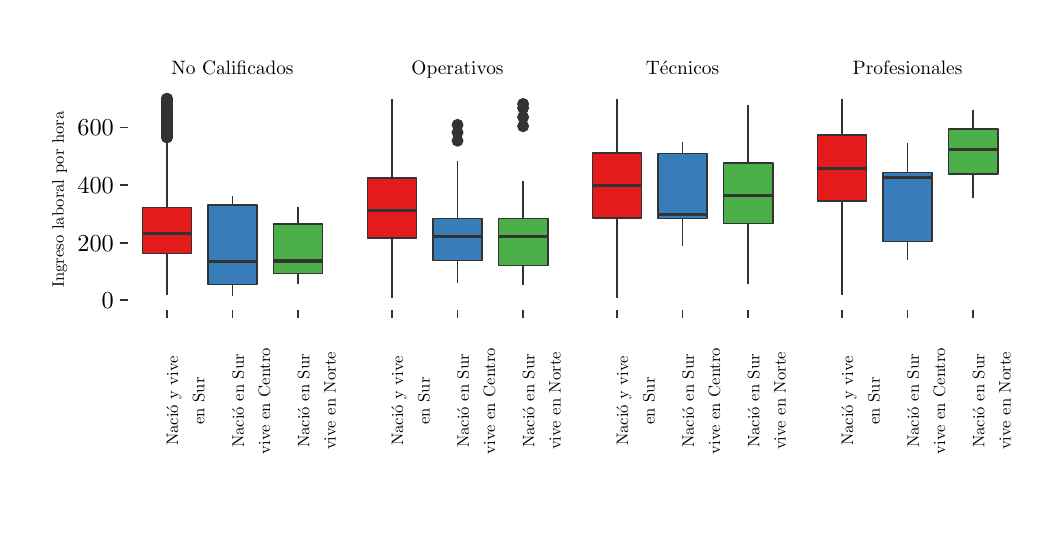
\begin{tikzpicture}[x=1pt,y=1pt]
\definecolor{fillColor}{RGB}{255,255,255}
\path[use as bounding box,fill=fillColor,fill opacity=0.00] (0,0) rectangle (361.35,180.67);
\begin{scope}
\path[clip] (  0.00,  0.00) rectangle (361.35,180.67);
\definecolor{drawColor}{RGB}{255,255,255}
\definecolor{fillColor}{RGB}{255,255,255}

\path[draw=drawColor,line width= 0.6pt,line join=round,line cap=round,fill=fillColor] (  0.00,  0.00) rectangle (361.35,180.68);
\end{scope}
\begin{scope}
\path[clip] ( 36.11, 78.54) rectangle (111.92,158.60);
\definecolor{drawColor}{RGB}{255,255,255}

\path[draw=drawColor,line width= 0.3pt,line join=round] ( 36.11, 92.57) --
	(111.92, 92.57);

\path[draw=drawColor,line width= 0.3pt,line join=round] ( 36.11,113.37) --
	(111.92,113.37);

\path[draw=drawColor,line width= 0.3pt,line join=round] ( 36.11,134.17) --
	(111.92,134.17);

\path[draw=drawColor,line width= 0.3pt,line join=round] ( 36.11,154.96) --
	(111.92,154.96);

\path[draw=drawColor,line width= 0.6pt,line join=round] ( 36.11, 82.18) --
	(111.92, 82.18);

\path[draw=drawColor,line width= 0.6pt,line join=round] ( 36.11,102.97) --
	(111.92,102.97);

\path[draw=drawColor,line width= 0.6pt,line join=round] ( 36.11,123.77) --
	(111.92,123.77);

\path[draw=drawColor,line width= 0.6pt,line join=round] ( 36.11,144.57) --
	(111.92,144.57);

\path[draw=drawColor,line width= 0.6pt,line join=round] ( 50.33, 78.54) --
	( 50.33,158.60);

\path[draw=drawColor,line width= 0.6pt,line join=round] ( 74.02, 78.54) --
	( 74.02,158.60);

\path[draw=drawColor,line width= 0.6pt,line join=round] ( 97.71, 78.54) --
	( 97.71,158.60);
\definecolor{drawColor}{gray}{0.20}
\definecolor{fillColor}{gray}{0.20}

\path[draw=drawColor,line width= 0.4pt,line join=round,line cap=round,fill=fillColor] ( 50.33,145.48) circle (  1.96);

\path[draw=drawColor,line width= 0.4pt,line join=round,line cap=round,fill=fillColor] ( 50.33,148.26) circle (  1.96);

\path[draw=drawColor,line width= 0.4pt,line join=round,line cap=round,fill=fillColor] ( 50.33,145.48) circle (  1.96);

\path[draw=drawColor,line width= 0.4pt,line join=round,line cap=round,fill=fillColor] ( 50.33,148.64) circle (  1.96);

\path[draw=drawColor,line width= 0.4pt,line join=round,line cap=round,fill=fillColor] ( 50.33,146.91) circle (  1.96);

\path[draw=drawColor,line width= 0.4pt,line join=round,line cap=round,fill=fillColor] ( 50.33,154.11) circle (  1.96);

\path[draw=drawColor,line width= 0.4pt,line join=round,line cap=round,fill=fillColor] ( 50.33,152.05) circle (  1.96);

\path[draw=drawColor,line width= 0.4pt,line join=round,line cap=round,fill=fillColor] ( 50.33,142.60) circle (  1.96);

\path[draw=drawColor,line width= 0.4pt,line join=round,line cap=round,fill=fillColor] ( 50.33,141.59) circle (  1.96);

\path[draw=drawColor,line width= 0.4pt,line join=round,line cap=round,fill=fillColor] ( 50.33,141.59) circle (  1.96);

\path[draw=drawColor,line width= 0.4pt,line join=round,line cap=round,fill=fillColor] ( 50.33,141.59) circle (  1.96);

\path[draw=drawColor,line width= 0.4pt,line join=round,line cap=round,fill=fillColor] ( 50.33,145.55) circle (  1.96);

\path[draw=drawColor,line width= 0.4pt,line join=round,line cap=round,fill=fillColor] ( 50.33,147.15) circle (  1.96);

\path[draw=drawColor,line width= 0.4pt,line join=round,line cap=round,fill=fillColor] ( 50.33,141.87) circle (  1.96);

\path[draw=drawColor,line width= 0.4pt,line join=round,line cap=round,fill=fillColor] ( 50.33,141.21) circle (  1.96);

\path[draw=drawColor,line width= 0.4pt,line join=round,line cap=round,fill=fillColor] ( 50.33,141.21) circle (  1.96);

\path[draw=drawColor,line width= 0.4pt,line join=round,line cap=round,fill=fillColor] ( 50.33,149.72) circle (  1.96);

\path[draw=drawColor,line width= 0.4pt,line join=round,line cap=round,fill=fillColor] ( 50.33,149.72) circle (  1.96);

\path[draw=drawColor,line width= 0.4pt,line join=round,line cap=round,fill=fillColor] ( 50.33,149.72) circle (  1.96);

\path[draw=drawColor,line width= 0.4pt,line join=round,line cap=round,fill=fillColor] ( 50.33,143.93) circle (  1.96);

\path[draw=drawColor,line width= 0.4pt,line join=round,line cap=round,fill=fillColor] ( 50.33,145.22) circle (  1.96);

\path[draw=drawColor,line width= 0.4pt,line join=round,line cap=round,fill=fillColor] ( 50.33,146.35) circle (  1.96);

\path[draw=drawColor,line width= 0.4pt,line join=round,line cap=round,fill=fillColor] ( 50.33,146.35) circle (  1.96);

\path[draw=drawColor,line width= 0.4pt,line join=round,line cap=round,fill=fillColor] ( 50.33,144.32) circle (  1.96);

\path[draw=drawColor,line width= 0.4pt,line join=round,line cap=round,fill=fillColor] ( 50.33,148.33) circle (  1.96);

\path[draw=drawColor,line width= 0.4pt,line join=round,line cap=round,fill=fillColor] ( 50.33,146.98) circle (  1.96);

\path[draw=drawColor,line width= 0.4pt,line join=round,line cap=round,fill=fillColor] ( 50.33,144.82) circle (  1.96);

\path[draw=drawColor,line width= 0.4pt,line join=round,line cap=round,fill=fillColor] ( 50.33,142.66) circle (  1.96);

\path[draw=drawColor,line width= 0.4pt,line join=round,line cap=round,fill=fillColor] ( 50.33,145.18) circle (  1.96);

\path[draw=drawColor,line width= 0.4pt,line join=round,line cap=round,fill=fillColor] ( 50.33,150.16) circle (  1.96);

\path[draw=drawColor,line width= 0.4pt,line join=round,line cap=round,fill=fillColor] ( 50.33,152.10) circle (  1.96);

\path[draw=drawColor,line width= 0.4pt,line join=round,line cap=round,fill=fillColor] ( 50.33,152.10) circle (  1.96);

\path[draw=drawColor,line width= 0.4pt,line join=round,line cap=round,fill=fillColor] ( 50.33,152.10) circle (  1.96);

\path[draw=drawColor,line width= 0.4pt,line join=round,line cap=round,fill=fillColor] ( 50.33,150.16) circle (  1.96);

\path[draw=drawColor,line width= 0.4pt,line join=round,line cap=round,fill=fillColor] ( 50.33,147.44) circle (  1.96);

\path[draw=drawColor,line width= 0.4pt,line join=round,line cap=round,fill=fillColor] ( 50.33,150.16) circle (  1.96);

\path[draw=drawColor,line width= 0.4pt,line join=round,line cap=round,fill=fillColor] ( 50.33,143.36) circle (  1.96);

\path[draw=drawColor,line width= 0.4pt,line join=round,line cap=round,fill=fillColor] ( 50.33,144.09) circle (  1.96);

\path[draw=drawColor,line width= 0.4pt,line join=round,line cap=round,fill=fillColor] ( 50.33,151.52) circle (  1.96);

\path[draw=drawColor,line width= 0.4pt,line join=round,line cap=round,fill=fillColor] ( 50.33,151.52) circle (  1.96);

\path[draw=drawColor,line width= 0.4pt,line join=round,line cap=round,fill=fillColor] ( 50.33,149.05) circle (  1.96);

\path[draw=drawColor,line width= 0.4pt,line join=round,line cap=round,fill=fillColor] ( 50.33,146.57) circle (  1.96);

\path[draw=drawColor,line width= 0.4pt,line join=round,line cap=round,fill=fillColor] ( 50.33,144.09) circle (  1.96);

\path[draw=drawColor,line width= 0.4pt,line join=round,line cap=round,fill=fillColor] ( 50.33,154.41) circle (  1.96);

\path[draw=drawColor,line width= 0.4pt,line join=round,line cap=round,fill=fillColor] ( 50.33,142.59) circle (  1.96);

\path[draw=drawColor,line width= 0.4pt,line join=round,line cap=round,fill=fillColor] ( 50.33,146.37) circle (  1.96);

\path[draw=drawColor,line width= 0.4pt,line join=round,line cap=round,fill=fillColor] ( 50.33,154.67) circle (  1.96);

\path[draw=drawColor,line width= 0.4pt,line join=round,line cap=round,fill=fillColor] ( 50.33,142.59) circle (  1.96);

\path[draw=drawColor,line width= 0.4pt,line join=round,line cap=round,fill=fillColor] ( 50.33,141.02) circle (  1.96);

\path[draw=drawColor,line width= 0.4pt,line join=round,line cap=round,fill=fillColor] ( 50.33,145.61) circle (  1.96);

\path[draw=drawColor,line width= 0.4pt,line join=round,line cap=round,fill=fillColor] ( 50.33,152.09) circle (  1.96);

\path[draw=drawColor,line width= 0.4pt,line join=round,line cap=round,fill=fillColor] ( 50.33,146.91) circle (  1.96);

\path[draw=drawColor,line width= 0.4pt,line join=round,line cap=round,fill=fillColor] ( 50.33,152.09) circle (  1.96);

\path[draw=drawColor,line width= 0.4pt,line join=round,line cap=round,fill=fillColor] ( 50.33,154.67) circle (  1.96);

\path[draw=drawColor,line width= 0.4pt,line join=round,line cap=round,fill=fillColor] ( 50.33,144.16) circle (  1.96);

\path[draw=drawColor,line width= 0.4pt,line join=round,line cap=round,fill=fillColor] ( 50.33,150.09) circle (  1.96);

\path[draw=drawColor,line width= 0.4pt,line join=round,line cap=round,fill=fillColor] ( 50.33,145.06) circle (  1.96);

\path[draw=drawColor,line width= 0.4pt,line join=round,line cap=round,fill=fillColor] ( 50.33,148.20) circle (  1.96);

\path[draw=drawColor,line width= 0.4pt,line join=round,line cap=round,fill=fillColor] ( 50.33,149.55) circle (  1.96);

\path[draw=drawColor,line width= 0.4pt,line join=round,line cap=round,fill=fillColor] ( 50.33,145.06) circle (  1.96);

\path[draw=drawColor,line width= 0.4pt,line join=round,line cap=round,fill=fillColor] ( 50.33,151.35) circle (  1.96);

\path[draw=drawColor,line width= 0.4pt,line join=round,line cap=round,fill=fillColor] ( 50.33,152.92) circle (  1.96);

\path[draw=drawColor,line width= 0.4pt,line join=round,line cap=round,fill=fillColor] ( 50.33,152.92) circle (  1.96);

\path[draw=drawColor,line width= 0.4pt,line join=round,line cap=round,fill=fillColor] ( 50.33,145.06) circle (  1.96);

\path[draw=drawColor,line width= 0.4pt,line join=round,line cap=round,fill=fillColor] ( 50.33,150.30) circle (  1.96);

\path[draw=drawColor,line width= 0.4pt,line join=round,line cap=round,fill=fillColor] ( 50.33,149.02) circle (  1.96);

\path[draw=drawColor,line width= 0.4pt,line join=round,line cap=round,fill=fillColor] ( 50.33,149.86) circle (  1.96);

\path[draw=drawColor,line width= 0.4pt,line join=round,line cap=round,fill=fillColor] ( 50.33,144.84) circle (  1.96);

\path[draw=drawColor,line width= 0.4pt,line join=round,line cap=round,fill=fillColor] ( 50.33,147.98) circle (  1.96);

\path[draw=drawColor,line width= 0.4pt,line join=round,line cap=round,fill=fillColor] ( 50.33,142.34) circle (  1.96);

\path[draw=drawColor,line width= 0.4pt,line join=round,line cap=round,fill=fillColor] ( 50.33,153.48) circle (  1.96);

\path[draw=drawColor,line width= 0.4pt,line join=round,line cap=round,fill=fillColor] ( 50.33,144.57) circle (  1.96);

\path[draw=drawColor,line width= 0.4pt,line join=round,line cap=round,fill=fillColor] ( 50.33,142.83) circle (  1.96);

\path[draw=drawColor,line width= 0.4pt,line join=round,line cap=round,fill=fillColor] ( 50.33,147.17) circle (  1.96);

\path[draw=drawColor,line width= 0.4pt,line join=round,line cap=round,fill=fillColor] ( 50.33,147.17) circle (  1.96);

\path[draw=drawColor,line width= 0.4pt,line join=round,line cap=round,fill=fillColor] ( 50.33,151.50) circle (  1.96);

\path[draw=drawColor,line width= 0.4pt,line join=round,line cap=round,fill=fillColor] ( 50.33,151.50) circle (  1.96);

\path[draw=drawColor,line width= 0.4pt,line join=round,line cap=round,fill=fillColor] ( 50.33,144.57) circle (  1.96);

\path[draw=drawColor,line width= 0.4pt,line join=round,line cap=round,fill=fillColor] ( 50.33,147.17) circle (  1.96);

\path[draw=drawColor,line width= 0.4pt,line join=round,line cap=round,fill=fillColor] ( 50.33,142.83) circle (  1.96);

\path[draw=drawColor,line width= 0.4pt,line join=round,line cap=round,fill=fillColor] ( 50.33,142.83) circle (  1.96);

\path[draw=drawColor,line width= 0.4pt,line join=round,line cap=round,fill=fillColor] ( 50.33,147.17) circle (  1.96);

\path[draw=drawColor,line width= 0.4pt,line join=round,line cap=round,fill=fillColor] ( 50.33,144.57) circle (  1.96);

\path[draw=drawColor,line width= 0.4pt,line join=round,line cap=round,fill=fillColor] ( 50.33,141.59) circle (  1.96);

\path[draw=drawColor,line width= 0.4pt,line join=round,line cap=round,fill=fillColor] ( 50.33,151.50) circle (  1.96);

\path[draw=drawColor,line width= 0.4pt,line join=round,line cap=round,fill=fillColor] ( 50.33,151.50) circle (  1.96);

\path[draw=drawColor,line width= 0.4pt,line join=round,line cap=round,fill=fillColor] ( 50.33,147.17) circle (  1.96);

\path[draw=drawColor,line width= 0.4pt,line join=round,line cap=round,fill=fillColor] ( 50.33,144.57) circle (  1.96);

\path[draw=drawColor,line width= 0.4pt,line join=round,line cap=round,fill=fillColor] ( 50.33,154.96) circle (  1.96);

\path[draw=drawColor,line width= 0.4pt,line join=round,line cap=round,fill=fillColor] ( 50.33,154.96) circle (  1.96);

\path[draw=drawColor,line width= 0.4pt,line join=round,line cap=round,fill=fillColor] ( 50.33,144.57) circle (  1.96);

\path[draw=drawColor,line width= 0.4pt,line join=round,line cap=round,fill=fillColor] ( 50.33,144.57) circle (  1.96);

\path[draw=drawColor,line width= 0.6pt,line join=round] ( 50.33,115.68) -- ( 50.33,140.46);

\path[draw=drawColor,line width= 0.6pt,line join=round] ( 50.33, 99.07) -- ( 50.33, 84.13);
\definecolor{fillColor}{RGB}{228,26,28}

\path[draw=drawColor,line width= 0.6pt,line join=round,line cap=round,fill=fillColor] ( 41.44,115.68) --
	( 41.44, 99.07) --
	( 59.21, 99.07) --
	( 59.21,115.68) --
	( 41.44,115.68) --
	cycle;

\path[draw=drawColor,line width= 1.1pt,line join=round] ( 41.44,106.34) -- ( 59.21,106.34);

\path[draw=drawColor,line width= 0.6pt,line join=round] ( 74.02,116.70) -- ( 74.02,119.91);

\path[draw=drawColor,line width= 0.6pt,line join=round] ( 74.02, 87.86) -- ( 74.02, 83.86);
\definecolor{fillColor}{RGB}{55,126,184}

\path[draw=drawColor,line width= 0.6pt,line join=round,line cap=round,fill=fillColor] ( 65.13,116.70) --
	( 65.13, 87.86) --
	( 82.90, 87.86) --
	( 82.90,116.70) --
	( 65.13,116.70) --
	cycle;

\path[draw=drawColor,line width= 1.1pt,line join=round] ( 65.13, 96.25) -- ( 82.90, 96.25);

\path[draw=drawColor,line width= 0.6pt,line join=round] ( 97.71,109.69) -- ( 97.71,115.78);

\path[draw=drawColor,line width= 0.6pt,line join=round] ( 97.71, 91.88) -- ( 97.71, 88.00);
\definecolor{fillColor}{RGB}{77,175,74}

\path[draw=drawColor,line width= 0.6pt,line join=round,line cap=round,fill=fillColor] ( 88.82,109.69) --
	( 88.82, 91.88) --
	(106.59, 91.88) --
	(106.59,109.69) --
	( 88.82,109.69) --
	cycle;

\path[draw=drawColor,line width= 1.1pt,line join=round] ( 88.82, 96.35) -- (106.59, 96.35);
\end{scope}
\begin{scope}
\path[clip] (117.42, 78.54) rectangle (193.23,158.60);
\definecolor{drawColor}{RGB}{255,255,255}

\path[draw=drawColor,line width= 0.3pt,line join=round] (117.42, 92.57) --
	(193.23, 92.57);

\path[draw=drawColor,line width= 0.3pt,line join=round] (117.42,113.37) --
	(193.23,113.37);

\path[draw=drawColor,line width= 0.3pt,line join=round] (117.42,134.17) --
	(193.23,134.17);

\path[draw=drawColor,line width= 0.3pt,line join=round] (117.42,154.96) --
	(193.23,154.96);

\path[draw=drawColor,line width= 0.6pt,line join=round] (117.42, 82.18) --
	(193.23, 82.18);

\path[draw=drawColor,line width= 0.6pt,line join=round] (117.42,102.97) --
	(193.23,102.97);

\path[draw=drawColor,line width= 0.6pt,line join=round] (117.42,123.77) --
	(193.23,123.77);

\path[draw=drawColor,line width= 0.6pt,line join=round] (117.42,144.57) --
	(193.23,144.57);

\path[draw=drawColor,line width= 0.6pt,line join=round] (131.64, 78.54) --
	(131.64,158.60);

\path[draw=drawColor,line width= 0.6pt,line join=round] (155.33, 78.54) --
	(155.33,158.60);

\path[draw=drawColor,line width= 0.6pt,line join=round] (179.02, 78.54) --
	(179.02,158.60);
\definecolor{drawColor}{gray}{0.20}

\path[draw=drawColor,line width= 0.6pt,line join=round] (131.64,126.28) -- (131.64,154.96);

\path[draw=drawColor,line width= 0.6pt,line join=round] (131.64,104.57) -- (131.64, 82.93);
\definecolor{fillColor}{RGB}{228,26,28}

\path[draw=drawColor,line width= 0.6pt,line join=round,line cap=round,fill=fillColor] (122.75,126.28) --
	(122.75,104.57) --
	(140.52,104.57) --
	(140.52,126.28) --
	(122.75,126.28) --
	cycle;

\path[draw=drawColor,line width= 1.1pt,line join=round] (122.75,114.68) -- (140.52,114.68);
\definecolor{fillColor}{gray}{0.20}

\path[draw=drawColor,line width= 0.4pt,line join=round,line cap=round,fill=fillColor] (155.33,145.55) circle (  1.96);

\path[draw=drawColor,line width= 0.4pt,line join=round,line cap=round,fill=fillColor] (155.33,142.82) circle (  1.96);

\path[draw=drawColor,line width= 0.4pt,line join=round,line cap=round,fill=fillColor] (155.33,139.82) circle (  1.96);

\path[draw=drawColor,line width= 0.6pt,line join=round] (155.33,111.71) -- (155.33,132.58);

\path[draw=drawColor,line width= 0.6pt,line join=round] (155.33, 96.58) -- (155.33, 88.25);
\definecolor{fillColor}{RGB}{55,126,184}

\path[draw=drawColor,line width= 0.6pt,line join=round,line cap=round,fill=fillColor] (146.44,111.71) --
	(146.44, 96.58) --
	(164.21, 96.58) --
	(164.21,111.71) --
	(146.44,111.71) --
	cycle;

\path[draw=drawColor,line width= 1.1pt,line join=round] (146.44,105.36) -- (164.21,105.36);
\definecolor{fillColor}{gray}{0.20}

\path[draw=drawColor,line width= 0.4pt,line join=round,line cap=round,fill=fillColor] (179.02,153.10) circle (  1.96);

\path[draw=drawColor,line width= 0.4pt,line join=round,line cap=round,fill=fillColor] (179.02,148.33) circle (  1.96);

\path[draw=drawColor,line width= 0.4pt,line join=round,line cap=round,fill=fillColor] (179.02,151.65) circle (  1.96);

\path[draw=drawColor,line width= 0.4pt,line join=round,line cap=round,fill=fillColor] (179.02,145.06) circle (  1.96);

\path[draw=drawColor,line width= 0.6pt,line join=round] (179.02,111.69) -- (179.02,125.34);

\path[draw=drawColor,line width= 0.6pt,line join=round] (179.02, 94.70) -- (179.02, 87.57);
\definecolor{fillColor}{RGB}{77,175,74}

\path[draw=drawColor,line width= 0.6pt,line join=round,line cap=round,fill=fillColor] (170.13,111.69) --
	(170.13, 94.70) --
	(187.90, 94.70) --
	(187.90,111.69) --
	(170.13,111.69) --
	cycle;

\path[draw=drawColor,line width= 1.1pt,line join=round] (170.13,105.05) -- (187.90,105.05);
\end{scope}
\begin{scope}
\path[clip] (198.73, 78.54) rectangle (274.54,158.60);
\definecolor{drawColor}{RGB}{255,255,255}

\path[draw=drawColor,line width= 0.3pt,line join=round] (198.73, 92.57) --
	(274.54, 92.57);

\path[draw=drawColor,line width= 0.3pt,line join=round] (198.73,113.37) --
	(274.54,113.37);

\path[draw=drawColor,line width= 0.3pt,line join=round] (198.73,134.17) --
	(274.54,134.17);

\path[draw=drawColor,line width= 0.3pt,line join=round] (198.73,154.96) --
	(274.54,154.96);

\path[draw=drawColor,line width= 0.6pt,line join=round] (198.73, 82.18) --
	(274.54, 82.18);

\path[draw=drawColor,line width= 0.6pt,line join=round] (198.73,102.97) --
	(274.54,102.97);

\path[draw=drawColor,line width= 0.6pt,line join=round] (198.73,123.77) --
	(274.54,123.77);

\path[draw=drawColor,line width= 0.6pt,line join=round] (198.73,144.57) --
	(274.54,144.57);

\path[draw=drawColor,line width= 0.6pt,line join=round] (212.94, 78.54) --
	(212.94,158.60);

\path[draw=drawColor,line width= 0.6pt,line join=round] (236.64, 78.54) --
	(236.64,158.60);

\path[draw=drawColor,line width= 0.6pt,line join=round] (260.33, 78.54) --
	(260.33,158.60);
\definecolor{drawColor}{gray}{0.20}

\path[draw=drawColor,line width= 0.6pt,line join=round] (212.94,135.32) -- (212.94,154.96);

\path[draw=drawColor,line width= 0.6pt,line join=round] (212.94,111.88) -- (212.94, 82.98);
\definecolor{fillColor}{RGB}{228,26,28}

\path[draw=drawColor,line width= 0.6pt,line join=round,line cap=round,fill=fillColor] (204.06,135.32) --
	(204.06,111.88) --
	(221.83,111.88) --
	(221.83,135.32) --
	(204.06,135.32) --
	cycle;

\path[draw=drawColor,line width= 1.1pt,line join=round] (204.06,123.50) -- (221.83,123.50);

\path[draw=drawColor,line width= 0.6pt,line join=round] (236.64,135.23) -- (236.64,139.28);

\path[draw=drawColor,line width= 0.6pt,line join=round] (236.64,111.69) -- (236.64,101.85);
\definecolor{fillColor}{RGB}{55,126,184}

\path[draw=drawColor,line width= 0.6pt,line join=round,line cap=round,fill=fillColor] (227.75,135.23) --
	(227.75,111.69) --
	(245.52,111.69) --
	(245.52,135.23) --
	(227.75,135.23) --
	cycle;

\path[draw=drawColor,line width= 1.1pt,line join=round] (227.75,113.07) -- (245.52,113.07);

\path[draw=drawColor,line width= 0.6pt,line join=round] (260.33,131.86) -- (260.33,152.66);

\path[draw=drawColor,line width= 0.6pt,line join=round] (260.33,109.90) -- (260.33, 88.22);
\definecolor{fillColor}{RGB}{77,175,74}

\path[draw=drawColor,line width= 0.6pt,line join=round,line cap=round,fill=fillColor] (251.44,131.86) --
	(251.44,109.90) --
	(269.21,109.90) --
	(269.21,131.86) --
	(251.44,131.86) --
	cycle;

\path[draw=drawColor,line width= 1.1pt,line join=round] (251.44,120.13) -- (269.21,120.13);
\end{scope}
\begin{scope}
\path[clip] (280.04, 78.54) rectangle (355.85,158.60);
\definecolor{drawColor}{RGB}{255,255,255}

\path[draw=drawColor,line width= 0.3pt,line join=round] (280.04, 92.57) --
	(355.85, 92.57);

\path[draw=drawColor,line width= 0.3pt,line join=round] (280.04,113.37) --
	(355.85,113.37);

\path[draw=drawColor,line width= 0.3pt,line join=round] (280.04,134.17) --
	(355.85,134.17);

\path[draw=drawColor,line width= 0.3pt,line join=round] (280.04,154.96) --
	(355.85,154.96);

\path[draw=drawColor,line width= 0.6pt,line join=round] (280.04, 82.18) --
	(355.85, 82.18);

\path[draw=drawColor,line width= 0.6pt,line join=round] (280.04,102.97) --
	(355.85,102.97);

\path[draw=drawColor,line width= 0.6pt,line join=round] (280.04,123.77) --
	(355.85,123.77);

\path[draw=drawColor,line width= 0.6pt,line join=round] (280.04,144.57) --
	(355.85,144.57);

\path[draw=drawColor,line width= 0.6pt,line join=round] (294.25, 78.54) --
	(294.25,158.60);

\path[draw=drawColor,line width= 0.6pt,line join=round] (317.95, 78.54) --
	(317.95,158.60);

\path[draw=drawColor,line width= 0.6pt,line join=round] (341.64, 78.54) --
	(341.64,158.60);
\definecolor{drawColor}{gray}{0.20}

\path[draw=drawColor,line width= 0.6pt,line join=round] (294.25,141.92) -- (294.25,154.96);

\path[draw=drawColor,line width= 0.6pt,line join=round] (294.25,118.14) -- (294.25, 83.99);
\definecolor{fillColor}{RGB}{228,26,28}

\path[draw=drawColor,line width= 0.6pt,line join=round,line cap=round,fill=fillColor] (285.37,141.92) --
	(285.37,118.14) --
	(303.14,118.14) --
	(303.14,141.92) --
	(285.37,141.92) --
	cycle;

\path[draw=drawColor,line width= 1.1pt,line join=round] (285.37,129.71) -- (303.14,129.71);

\path[draw=drawColor,line width= 0.6pt,line join=round] (317.95,128.29) -- (317.95,138.88);

\path[draw=drawColor,line width= 0.6pt,line join=round] (317.95,103.40) -- (317.95, 96.61);
\definecolor{fillColor}{RGB}{55,126,184}

\path[draw=drawColor,line width= 0.6pt,line join=round,line cap=round,fill=fillColor] (309.06,128.29) --
	(309.06,103.40) --
	(326.83,103.40) --
	(326.83,128.29) --
	(309.06,128.29) --
	cycle;

\path[draw=drawColor,line width= 1.1pt,line join=round] (309.06,126.50) -- (326.83,126.50);

\path[draw=drawColor,line width= 0.6pt,line join=round] (341.64,144.02) -- (341.64,151.05);

\path[draw=drawColor,line width= 0.6pt,line join=round] (341.64,127.71) -- (341.64,119.07);
\definecolor{fillColor}{RGB}{77,175,74}

\path[draw=drawColor,line width= 0.6pt,line join=round,line cap=round,fill=fillColor] (332.75,144.02) --
	(332.75,127.71) --
	(350.52,127.71) --
	(350.52,144.02) --
	(332.75,144.02) --
	cycle;

\path[draw=drawColor,line width= 1.1pt,line join=round] (332.75,136.56) -- (350.52,136.56);
\end{scope}
\begin{scope}
\path[clip] ( 36.11,158.60) rectangle (111.92,175.17);
\definecolor{drawColor}{RGB}{0,0,0}

\node[text=drawColor,anchor=base,inner sep=0pt, outer sep=0pt, scale=  0.70] at ( 74.02,163.86) {No Calificados};
\end{scope}
\begin{scope}
\path[clip] (117.42,158.60) rectangle (193.23,175.17);
\definecolor{drawColor}{RGB}{0,0,0}

\node[text=drawColor,anchor=base,inner sep=0pt, outer sep=0pt, scale=  0.70] at (155.33,163.86) {Operativos};
\end{scope}
\begin{scope}
\path[clip] (198.73,158.60) rectangle (274.54,175.17);
\definecolor{drawColor}{RGB}{0,0,0}

\node[text=drawColor,anchor=base,inner sep=0pt, outer sep=0pt, scale=  0.70] at (236.64,163.86) {Técnicos};
\end{scope}
\begin{scope}
\path[clip] (280.04,158.60) rectangle (355.85,175.17);
\definecolor{drawColor}{RGB}{0,0,0}

\node[text=drawColor,anchor=base,inner sep=0pt, outer sep=0pt, scale=  0.70] at (317.95,163.86) {Profesionales};
\end{scope}
\begin{scope}
\path[clip] (  0.00,  0.00) rectangle (361.35,180.67);
\definecolor{drawColor}{gray}{0.20}

\path[draw=drawColor,line width= 0.6pt,line join=round] ( 50.33, 75.79) --
	( 50.33, 78.54);

\path[draw=drawColor,line width= 0.6pt,line join=round] ( 74.02, 75.79) --
	( 74.02, 78.54);

\path[draw=drawColor,line width= 0.6pt,line join=round] ( 97.71, 75.79) --
	( 97.71, 78.54);
\end{scope}
\begin{scope}
\path[clip] (  0.00,  0.00) rectangle (361.35,180.67);
\definecolor{drawColor}{RGB}{0,0,0}

\node[text=drawColor,rotate= 90.00,anchor=base,inner sep=0pt, outer sep=0pt, scale=  0.60] at ( 54.39, 45.78) {Nació y vive};

\node[text=drawColor,rotate= 90.00,anchor=base,inner sep=0pt, outer sep=0pt, scale=  0.60] at ( 63.89, 45.78) {en Sur};

\node[text=drawColor,rotate= 90.00,anchor=base,inner sep=0pt, outer sep=0pt, scale=  0.60] at ( 78.08, 45.78) {Nació en Sur};

\node[text=drawColor,rotate= 90.00,anchor=base,inner sep=0pt, outer sep=0pt, scale=  0.60] at ( 87.58, 45.78) {vive en Centro};

\node[text=drawColor,rotate= 90.00,anchor=base,inner sep=0pt, outer sep=0pt, scale=  0.60] at (101.77, 45.78) {Nació en Sur};

\node[text=drawColor,rotate= 90.00,anchor=base,inner sep=0pt, outer sep=0pt, scale=  0.60] at (111.27, 45.78) {vive en Norte};
\end{scope}
\begin{scope}
\path[clip] (  0.00,  0.00) rectangle (361.35,180.67);
\definecolor{drawColor}{gray}{0.20}

\path[draw=drawColor,line width= 0.6pt,line join=round] (131.64, 75.79) --
	(131.64, 78.54);

\path[draw=drawColor,line width= 0.6pt,line join=round] (155.33, 75.79) --
	(155.33, 78.54);

\path[draw=drawColor,line width= 0.6pt,line join=round] (179.02, 75.79) --
	(179.02, 78.54);
\end{scope}
\begin{scope}
\path[clip] (  0.00,  0.00) rectangle (361.35,180.67);
\definecolor{drawColor}{RGB}{0,0,0}

\node[text=drawColor,rotate= 90.00,anchor=base,inner sep=0pt, outer sep=0pt, scale=  0.60] at (135.70, 45.78) {Nació y vive};

\node[text=drawColor,rotate= 90.00,anchor=base,inner sep=0pt, outer sep=0pt, scale=  0.60] at (145.20, 45.78) {en Sur};

\node[text=drawColor,rotate= 90.00,anchor=base,inner sep=0pt, outer sep=0pt, scale=  0.60] at (159.39, 45.78) {Nació en Sur};

\node[text=drawColor,rotate= 90.00,anchor=base,inner sep=0pt, outer sep=0pt, scale=  0.60] at (168.89, 45.78) {vive en Centro};

\node[text=drawColor,rotate= 90.00,anchor=base,inner sep=0pt, outer sep=0pt, scale=  0.60] at (183.08, 45.78) {Nació en Sur};

\node[text=drawColor,rotate= 90.00,anchor=base,inner sep=0pt, outer sep=0pt, scale=  0.60] at (192.58, 45.78) {vive en Norte};
\end{scope}
\begin{scope}
\path[clip] (  0.00,  0.00) rectangle (361.35,180.67);
\definecolor{drawColor}{gray}{0.20}

\path[draw=drawColor,line width= 0.6pt,line join=round] (212.94, 75.79) --
	(212.94, 78.54);

\path[draw=drawColor,line width= 0.6pt,line join=round] (236.64, 75.79) --
	(236.64, 78.54);

\path[draw=drawColor,line width= 0.6pt,line join=round] (260.33, 75.79) --
	(260.33, 78.54);
\end{scope}
\begin{scope}
\path[clip] (  0.00,  0.00) rectangle (361.35,180.67);
\definecolor{drawColor}{RGB}{0,0,0}

\node[text=drawColor,rotate= 90.00,anchor=base,inner sep=0pt, outer sep=0pt, scale=  0.60] at (217.01, 45.78) {Nació y vive};

\node[text=drawColor,rotate= 90.00,anchor=base,inner sep=0pt, outer sep=0pt, scale=  0.60] at (226.51, 45.78)  {en Sur};

\node[text=drawColor,rotate= 90.00,anchor=base,inner sep=0pt, outer sep=0pt, scale=  0.60] at (240.70, 45.78)  {Nació en Sur};

\node[text=drawColor,rotate= 90.00,anchor=base,inner sep=0pt, outer sep=0pt, scale=  0.60] at (250.20, 45.78) {vive en Centro};

\node[text=drawColor,rotate= 90.00,anchor=base,inner sep=0pt, outer sep=0pt, scale=  0.60] at (264.39, 45.78) {Nació en Sur};

\node[text=drawColor,rotate= 90.00,anchor=base,inner sep=0pt, outer sep=0pt, scale=  0.60] at (273.89, 45.78) {vive en Norte};
\end{scope}
\begin{scope}
\path[clip] (  0.00,  0.00) rectangle (361.35,180.67);
\definecolor{drawColor}{gray}{0.20}

\path[draw=drawColor,line width= 0.6pt,line join=round] (294.25, 75.79) --
	(294.25, 78.54);

\path[draw=drawColor,line width= 0.6pt,line join=round] (317.95, 75.79) --
	(317.95, 78.54);

\path[draw=drawColor,line width= 0.6pt,line join=round] (341.64, 75.79) --
	(341.64, 78.54);
\end{scope}
\begin{scope}
\path[clip] (  0.00,  0.00) rectangle (361.35,180.67);
\definecolor{drawColor}{RGB}{0,0,0}

\node[text=drawColor,rotate= 90.00,anchor=base,inner sep=0pt, outer sep=0pt, scale=  0.60] at (298.32, 45.78) {Nació y vive};

\node[text=drawColor,rotate= 90.00,anchor=base,inner sep=0pt, outer sep=0pt, scale=  0.60] at (307.82, 45.78) {en Sur};

\node[text=drawColor,rotate= 90.00,anchor=base,inner sep=0pt, outer sep=0pt, scale=  0.60] at (322.01, 45.78) {Nació en Sur};

\node[text=drawColor,rotate= 90.00,anchor=base,inner sep=0pt, outer sep=0pt, scale=  0.60] at (331.51, 45.78) {vive en Centro};

\node[text=drawColor,rotate= 90.00,anchor=base,inner sep=0pt, outer sep=0pt, scale=  0.60] at (345.70, 45.78) {Nació en Sur};

\node[text=drawColor,rotate= 90.00,anchor=base,inner sep=0pt, outer sep=0pt, scale=  0.60] at (355.20, 45.78) {vive en Norte};
\end{scope}
\begin{scope}
\path[clip] (  0.00,  0.00) rectangle (361.35,180.67);
\definecolor{drawColor}{RGB}{0,0,0}

\node[text=drawColor,anchor=base east,inner sep=0pt, outer sep=0pt, scale=  0.88] at ( 31.16, 79.15) {0};

\node[text=drawColor,anchor=base east,inner sep=0pt, outer sep=0pt, scale=  0.88] at ( 31.16, 99.94) {200};

\node[text=drawColor,anchor=base east,inner sep=0pt, outer sep=0pt, scale=  0.88] at ( 31.16,120.74) {400};

\node[text=drawColor,anchor=base east,inner sep=0pt, outer sep=0pt, scale=  0.88] at ( 31.16,141.54) {600};
\end{scope}
\begin{scope}
\path[clip] (  0.00,  0.00) rectangle (361.35,180.67);
\definecolor{drawColor}{gray}{0.20}

\path[draw=drawColor,line width= 0.6pt,line join=round] ( 33.36, 82.18) --
	( 36.11, 82.18);

\path[draw=drawColor,line width= 0.6pt,line join=round] ( 33.36,102.97) --
	( 36.11,102.97);

\path[draw=drawColor,line width= 0.6pt,line join=round] ( 33.36,123.77) --
	( 36.11,123.77);

\path[draw=drawColor,line width= 0.6pt,line join=round] ( 33.36,144.57) --
	( 36.11,144.57);
\end{scope}
\begin{scope}
\path[clip] (  0.00,  0.00) rectangle (361.35,180.67);
\definecolor{drawColor}{RGB}{0,0,0}

\node[text=drawColor,rotate= 90.00,anchor=base,inner sep=0pt, outer sep=0pt, scale=  0.6] at ( 13.08,118.57) {Ingreso laboral por hora};
\end{scope}
\end{tikzpicture}
